\chapter{\texorpdfstring{\ds and \dpl signal extraction}{Ds+ and D+ signal extraction}}

The main ingredient for the evaluation of the \ds/\dpl production-yield ratio is the \ds and \dpl raw yield, i.e., the number of reconstructed \ds and \dpl mesons. Due to the vast amount of combinatorial background and the limited efficiency of about 1\%, the extraction of the raw yield is not possible through a candidate counting method. Instead, the raw yield is obtained on a statistical basis by fitting the invariant-mass distribution of the \ds and \dpl candidates passing tight selection criteria. To reduce the combinatorial background and enhance the efficiency of D-meson selection, Machine Learning algorithms have been employed. The following sections describe the procedure for the extraction of the raw yield of \ds and \dpl mesons. 

\section{Machine Learning}
The term \emph{Machine Learning} (ML) is a broad and versatile concept, encompassing a wide range of algorithms that grant computers the capacity to learn and adapt without being explicitly programmed to do so~\cite{5392560}. A more comprehensive definition characterises ML as the study of algorithms that enhance their performance (P) at a specific task (T) through the accumulation of experience (E)~\cite{mitchell1997machine}. In recent years, ML techniques have witnessed widespread adoption across diverse fields, with significant impacts realised especially with the emergence of generative models such as GPT~\cite{openai2023gpt4}.
ML algorithms have found extensive applications in the high-energy physics field, primarily for the task of distinguishing interesting signals from the vast background present in particle collision data. Furthermore, these algorithms have been employed as triggers, aiding in the rapid identification of events of interest, and have also been instrumental in event reconstruction. Notably, ML algorithms were used in the discovery of the Higgs boson~\cite{CMS:2012qbp}, one of the most significant achievements in the field of particle physics. \textcolor{red}{Aggiungere che permette di fare selezioni non lineari}

\subsection{Supervised learning}
Supervised learning is one of the main branches of machine-learning problems, together with unsupervised and reinforcement learning. Machine learning tasks are usually described in terms of how the machine learning system should process an example, which is a collection of features $\mathbf{x}$ that have been quantitatively measured from some object or event that one wants the machine learning system to process. In the case of supervised learning, each example is coupled with a corresponding label or target, $\mathbf{y}$. The objective of supervised learning is to learn to predict or infer $\mathbf{y}$ based on the associated features, $\mathbf{x}$, assuming that there exists a functional relationship $\mathbf{y} = f(\mathbf{x})$ between the two. The goal of the machine learning system is to produce an approximation $\widehat{f}(\mathbf{x})$ of the true function $f(\mathbf{x})$ by minimising a given loss function, which quantifies the discrepancy between the predicted and true labels. Supervised learning problems exhibit further segmentation into two distinct sub-categories, known as classification and regression. In the former, the label $\mathbf{y}$ assumes values from a finite and discrete set of categories, often representing distinct classes or groups. In the latter, the label $\mathbf{y}$ takes the form of one or more continuous variables. This necessitates the learning system to deduce a continuous function or mapping between $\mathbf{x}$ and $\mathbf{y}$, where the goal is to predict and approximate numerical values or class affiliations.

The application of a supervised learning algorithm to a dataset involves the following steps: i. the model is trained on a set of labelled data, i.e., the value of $\mathbf{y}$ is known for each example in the training set; ii. the model is tested on a separate set of labelled data, known as the test set, to evaluate its performance; iii. the model is then used to make predictions on new, unseen data.

\subsubsection{Training}
During the training process, the model learns (i.e., adjusts its internal parameters) to map the input features $\mathbf{x}$ to the corresponding labels $\mathbf{y}$ by minimizing a given loss function. Typically used loss functions include the Mean Squared Error (MSE) for regression tasks and the Cross-Entropy loss for classification tasks. The loss function is minimised through an optimization algorithm, usually stochastic gradient descent~\cite{10.1214/aoms/1177729392}, which iteratively updates the model parameters to reduce the loss. Since an overoptimisation of the model on the training data can lead to poor generalization on unseen data (the model is said to be \emph{overfitting}), a regularisation term is often added to the loss function to penalise overly complex models. The training process continues until the model reaches a satisfactory level of performance on the training data, or until its performance does not improve further. 

Before the final model training, hyperparameters tuning is performed to optimise the model's performance. \emph{Hyperparameters} are parameters that are not learned during the training process, but rather define the model's architecture and the training process itself. Hyperparameters tuning is usually performed through a grid search or random search\textcolor{red}{aggiungere bayesian}, where different combinations of hyperparameters are tested on a dedicated labelled dataset, different from the training set: the validation set. Models with different hyperparameter sets are trained with a reduced training phase, and those yielding the best performance are then selected for the final model training.

\subsubsection{Testing}
After the model has been trained, its performance is evaluated on a dataset that was not used during the training process, known as the test set. Like the training and validation sets, also the test set contains labelled examples. While during the training the model is optimised to minimise the loss function, the test set is used to estimate the model's generalization error, i.e., how well the model performs on unseen data. The model's performance is evaluated using metrics that are specific to the task at hand, such as accuracy for classification tasks, or Mean Squared Error (MSE) for regression tasks. Once the model achieves satisfactory performance on the test set, it is ready to be used for making predictions on unlabelled data.

\subsubsection{Cross-validation}

With the strategy defined above to optimise the hyperparameters, train the model and validate its performance, the dataset is divided into three subsets: the training set, the validation set, and the test set. When small datasets are involved, this division can lead to a suboptimal model, as the model's performance can be highly dependent on the specific examples in the training, validation, and test sets. Furthermore, this approach limits the amount of data available for training the model, which can lead to poor generalization. To mitigate this issue, a technique called cross-validation is often employed. It consists on dividing the training sample into $k$ subsets of equal size, called \emph{folds}. Then, the ML algorithm is trained $k$ times, each time using $k-1$ folds as training set, while the remaining fold is used as validation set. The model's performance is then averaged over the $k$ folds to obtain a more robust estimate of this quantity. This operation is repeated for each hyperparameter configuration to be considered. The hyperparameter configuration minimising the loss function is then chosen as the optimal configuration.

\section{\texorpdfstring{\ds and \dpl selection using Machine Learning}{Ds+ and D+ selection using Machine Learning}}

The task of extracting \ds and \dpl signals from the vast combinatorial background is a challenging one, due to the large amount of background compared to signal. It is however an excellent example of classification problem, and ML algorithms can therefore be exploited to enhance the efficiency of the selection. 

\subsection{Data preparation}
\textcolor{red}{Aggiungere come settiamo le labels (0=bkg, 1 = prompt, 2= FD)}
In order to train a ML model, a labelled dataset with a well defined set of features is required. The dataset is composed of signal and background examples. To obtain a pure sample of signal candidates, Monte Carlo simulations are used to generate \ds and \dpl mesons. Proton-proton collisions are generated using the \textsc{Pythia~8} event generator~\cite{Bierlich:2022pfr} with colour-reconnection Mode~2~\cite{Christiansen:2015yqa}, and the generated particles are propagated through the ALICE detector using the \textsc{Geant4} transport simulation toolkit~\cite{GEANT4:2002zbu}. To enrich the sample of heavy-flavour hadrons, $\mathrm{c\overline{c}}$ and $\mathrm{b\overline{b}}$ pairs are injected into each simulated event. 


%Due to the displaced topology of heavy-flavour decays and the continuous readout employed by the ALICE detector, the selection of events with charm or beauty hadrons produces ``fake'' vertices arising from the association of displaced decay tracks, affecting the reconstruction of heavy-flavour hadrons. To overcome this problem, minimum bias events are generated between charm or beauty enriched ones (\emph{gap-triggered} approach). Studies performed using different gap sizes have shown that a gap of 5 minimum bias events reduces the fake-vertex rate to an acceptable level, while keeping the simulation time reasonable. 

Only prompt and non-prompt \ds mesons are used to train the model, as \dpl mesons decay into the same final state as \ds mesons, and selections optimised to reconstruct \ds mesons are also effective for \dpl mesons. 

Background candidates are obtained from real data, as MC simulations may not able to reproduce the complexity of soft processes occurring in the underlying event, or may not be able to model the detector response accurately. The background examples are obtained by selecting candidates from a subsample of the full data sample (correspondig to its 3\%) in an invariant-mass region away from both the \ds and \dpl mass peaks, where $1.7 < M < 1.75$~\gevcc or \mbox{$2.1 < M < 2.15$~\gevcc}, as shown in Fig.~\ref{fig:ml_training_mass}. 

\begin{figure}[htb]
    \centering
    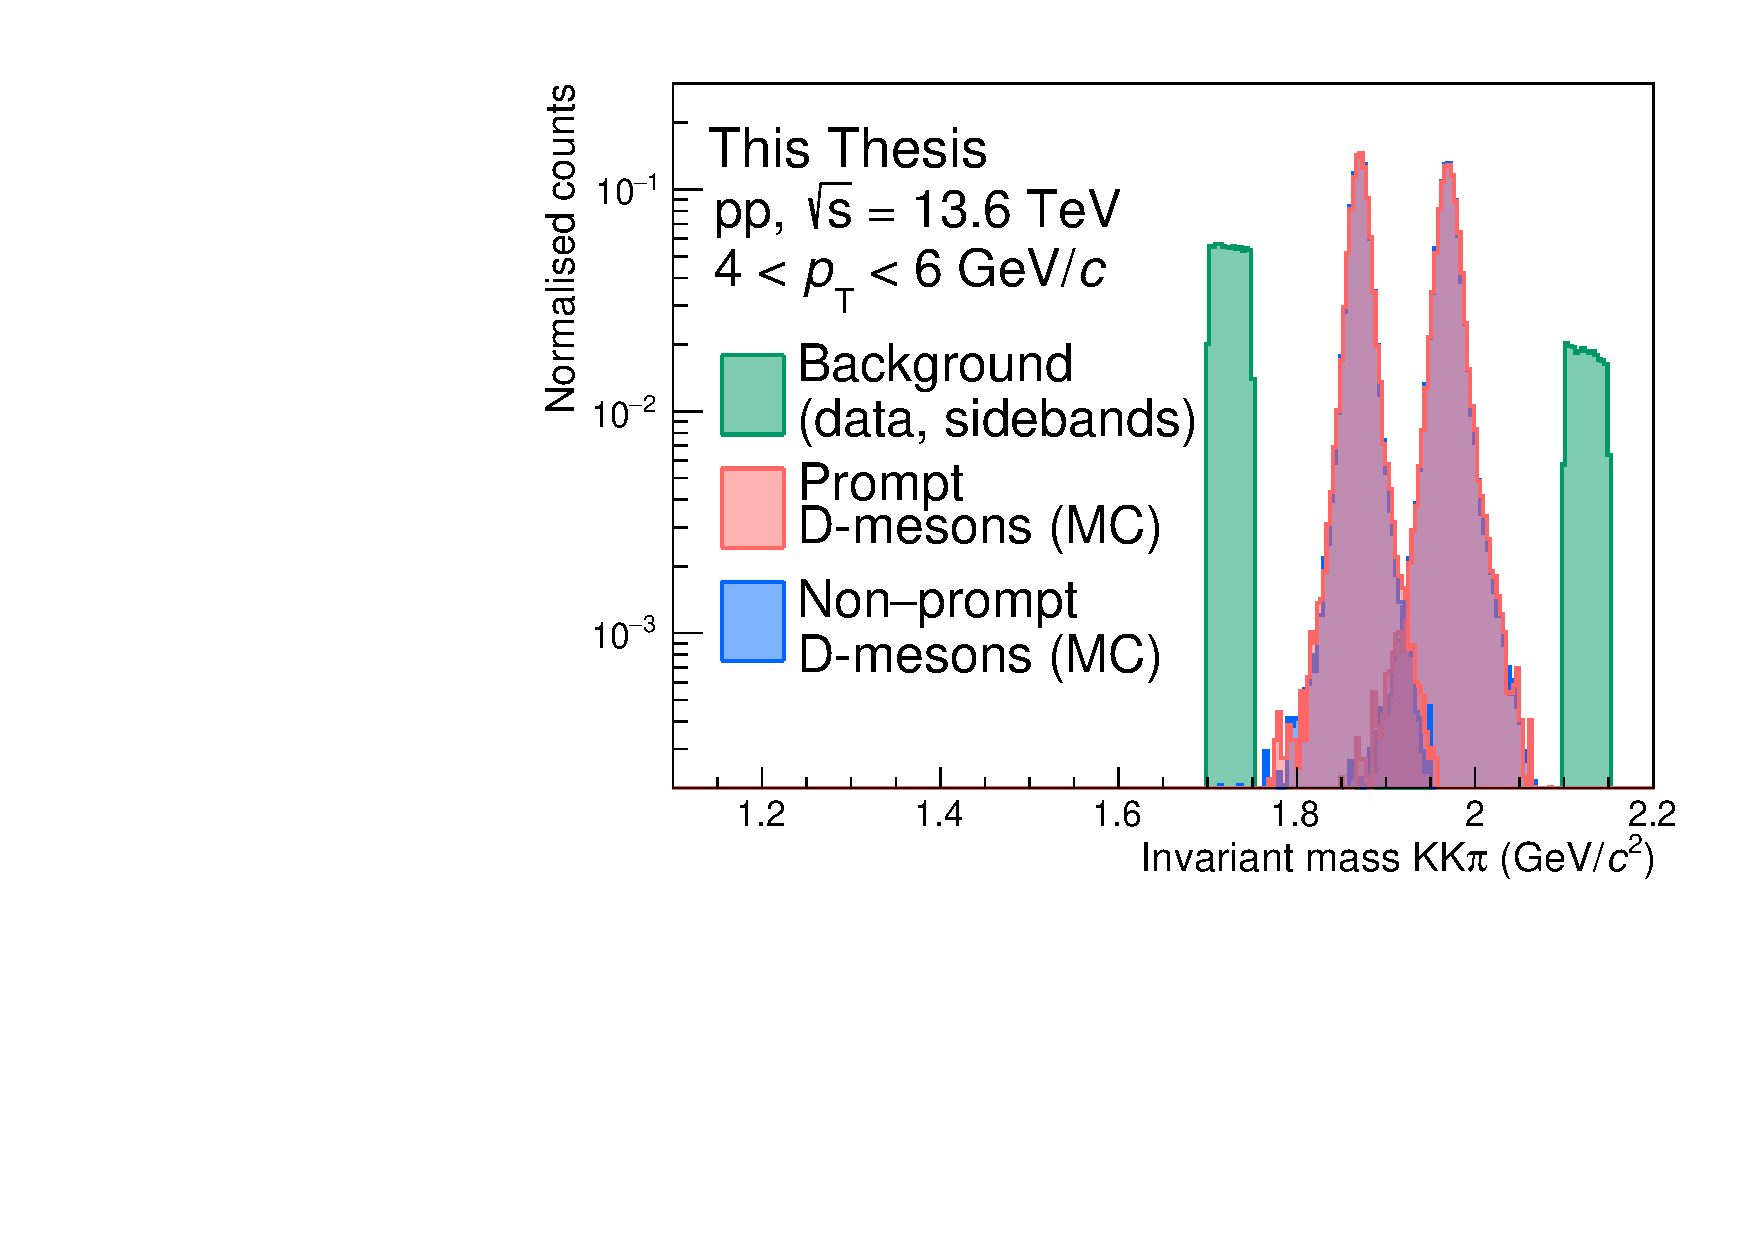
\includegraphics[width=0.7\textwidth]{Figures/Chapter 5/Mass.pdf}
    \caption{Invariant mass distribution of the backgound candidates used to train the ML model (green) and of prompt and non-prompt D-mesons (blue and orange, respectively), taken from Monte Carlo simulations, in the $4<\pt<6$~\gevc interval. Background candidates are selected in the $1.7 < M < 1.75$~\gevcc or \mbox{$2.1 < M < 2.15$~\gevcc} invariant-mass interval.}
    \label{fig:ml_training_mass}
\end{figure}

The dataset is then divided into two different subsamples. The first comprehends 80\% of the data, and is used to train the model, while the remaining 20\% is used to test its performance. In addition, since the D-mesons decay topology can significantly differ depending on the \pt of the meson due to different Lorentz boosts, the dataset is divided into several \pt intervals, and the model is trained and tested separately for each of them. The total number of candidates availabe for training and testing the model is reported in Table~\ref{tab:training_sample} for the considered \pt intervals.


\begin{table}[htb]
    \begin{center}
    \caption{Number of candidates within the \pt intervals used to train and test the model.}
    \label{tab:training_sample}
    \vspace*{0.3cm}
    \begin{tabular}{c|ccc}
         \toprule
         \pt (\gevc) & Prompt \ds & Non-prompt \ds & Background\\
         \midrule         
         0--1.5     & $\sim 4.6 \times 10^{3}$  & $\sim 21  \times 10^{3}$   & $\sim 726  \times 10^{3}$ \\
         1.5--2     & $\sim 6.1 \times 10^{3}$  & $\sim 24  \times 10^{3}$   & $\sim 92   \times 10^{3}$\\
         2--3       & $\sim 26  \times 10^{3}$  & $\sim 96  \times 10^{3}$   & $\sim 123  \times 10^{3}$ \\
         3--4       & $\sim 34  \times 10^{3}$  & $\sim 124 \times 10^{3}$   & $\sim 114  \times 10^{3}$ \\
         4--5       & $\sim 31  \times 10^{3}$  & $\sim 113 \times 10^{3}$   & $\sim 63   \times 10^{3}$\\
         5--6       & $\sim 24  \times 10^{3}$  & $\sim 89  \times 10^{3}$   & $\sim 29   \times 10^{3}$\\
         6--8       & $\sim 32  \times 10^{3}$  & $\sim 115 \times 10^{3}$   & $\sim 22   \times 10^{3}$\\
         8--12      & $\sim 23  \times 10^{3}$  & $\sim 89  \times 10^{3}$   & $\sim 10   \times 10^{3}$\\
         12--24     & $\sim 9.7 \times 10^{3}$  & $\sim 39  \times 10^{3}$   & $\sim 2.6  \times 10^{3}$ \\
         \bottomrule
    \end{tabular}
    \end{center}
\end{table}

\begin{sloppypar}
To produce a balanced dataset, the number of candidates in each class is equalised to the number of examples in the minority class. This is achieved by randomly selecting a subset of the majority classes. The balanced dataset is then used to train the model.
\end{sloppypar}

The choice of features used to separate signal from background is crucial, as they must be able to discriminate between signal and background candidates, and must be chosen in such a way that no bias is introduced in the final result. The variables used to train the model were introduced in Chapter~\ref{chap:reconstruction}, and are a mix of topological, kinematic, and PID variables. The key idea is to exploit the displaced topology of the D-meson decay, which is a distinctive feature of the signal candidates, the kinematic properties of the D-meson decay, and the PID information of the daughter tracks to discriminate between signal and background candidates. The features used to train the model are reported in Table~\ref{tab:ml_training_vars}. The number in parenthesis after $n\sigma$ indicates the prong number.

\begin{table}[htb]
    \begin{center}
    \caption{Candidate features used to train the ML model.}
    \label{tab:ml_training_vars}
    \vspace*{0.3cm}
    \begin{tabular}{c}
         \toprule
         Variable\\
         \midrule         
         cos$\theta_{p}$\\
         cos$\theta_{p}^{xy}$\\
         Decay length\\
         Decay length XY\\
         Candidate impact parameter XY\\
         $\lvert \cos^{3}\theta'(\mathrm K)\rvert$\\
         Prong 0 impact parameter XY\\
         Prong 1 impact parameter XY\\
         Prong 2 impact parameter XY\\
         $n\sigma_{\mathrm comb}^{\pi}(0)$\\         
         $n\sigma_{\mathrm comb}^{\pi}(1)$\\
         $n\sigma_{\mathrm comb}^{\pi}(2)$\\
         $n\sigma_{\mathrm comb}^{\mathrm K}(0)$\\
         $n\sigma_{\mathrm comb}^{\mathrm K}(1)$\\
         $n\sigma_{\mathrm comb}^{\mathrm K}(2)$\\
         \bottomrule
    \end{tabular}
    \end{center}
\end{table}

The invariant mass of the candidate and its \pt are not used to train the model. Exploiting such variables would introduce a bias in the final result, as the model would be trained to select candidates within a specific invariant mass region (that of \ds and \dpl mesons) or \pt. This would affect both the selection of the candidates and the \pt distribution of the final sample, leading to a biased \pt-differential yield. However, some of the variables used to train the model may be correlated with the invariant mass of the candidate, and the ML may learn to discriminate the signal from the background by exploiting the correlation with the \ds meson mass and transverse momentum, rather than the physical properties of the signal and background. To exclude this possibility, the correlation between the features used to train the model is studied. To quantitatively describe the correlation between the variables, the Pearson correlation coefficient $\rho$ is evaluated for each pair of variables. It is defined as the ratio between the covariance of two variables and the product of their standard deviations, $\rho(x,y) = \mathrm{cov}(x,y)/(\sigma_{x}\sigma_{y})$. It expresses the strength and direction of a linear correlation between two variables, ranging from $\rho = 1$ (perfect positive linear correlation) to $\rho = -1$ (perfect negative linear relationship). $\rho = 0$ indicates no linear correlation.

The correlation matrix of the features used to train the model is shown in Fig.~\ref{fig:ml_training_vars} for the prompt \ds, non-prompt \ds and background classes, in the $2<\pt<3$~\gevc. The correlation with the invariant mass and the transverse momentum is also reported. The Pearson coefficient is encoded in the colour of the cell, with red indicating a positive correlation, blue a negative correlation, and grey no correlation. The correlation matrix shows that the variables used to train the model are not correlated with the invariant mass of the candidate, suggesting that a ML should not modify the invariant-mass distribution of the selected candidates, which would introduce a bias in the measurement.

Variables carrying the same physical information, such as those related to the candidate decay length, pointing angle, and impact parameter, are strongly correlated among each other, as expected. Different degrees of correlation between the same variables in the different classes are observed. The ML model can exploit these differences to discriminate between signal and background candidates.

\begin{figure}[p]
    \centering
    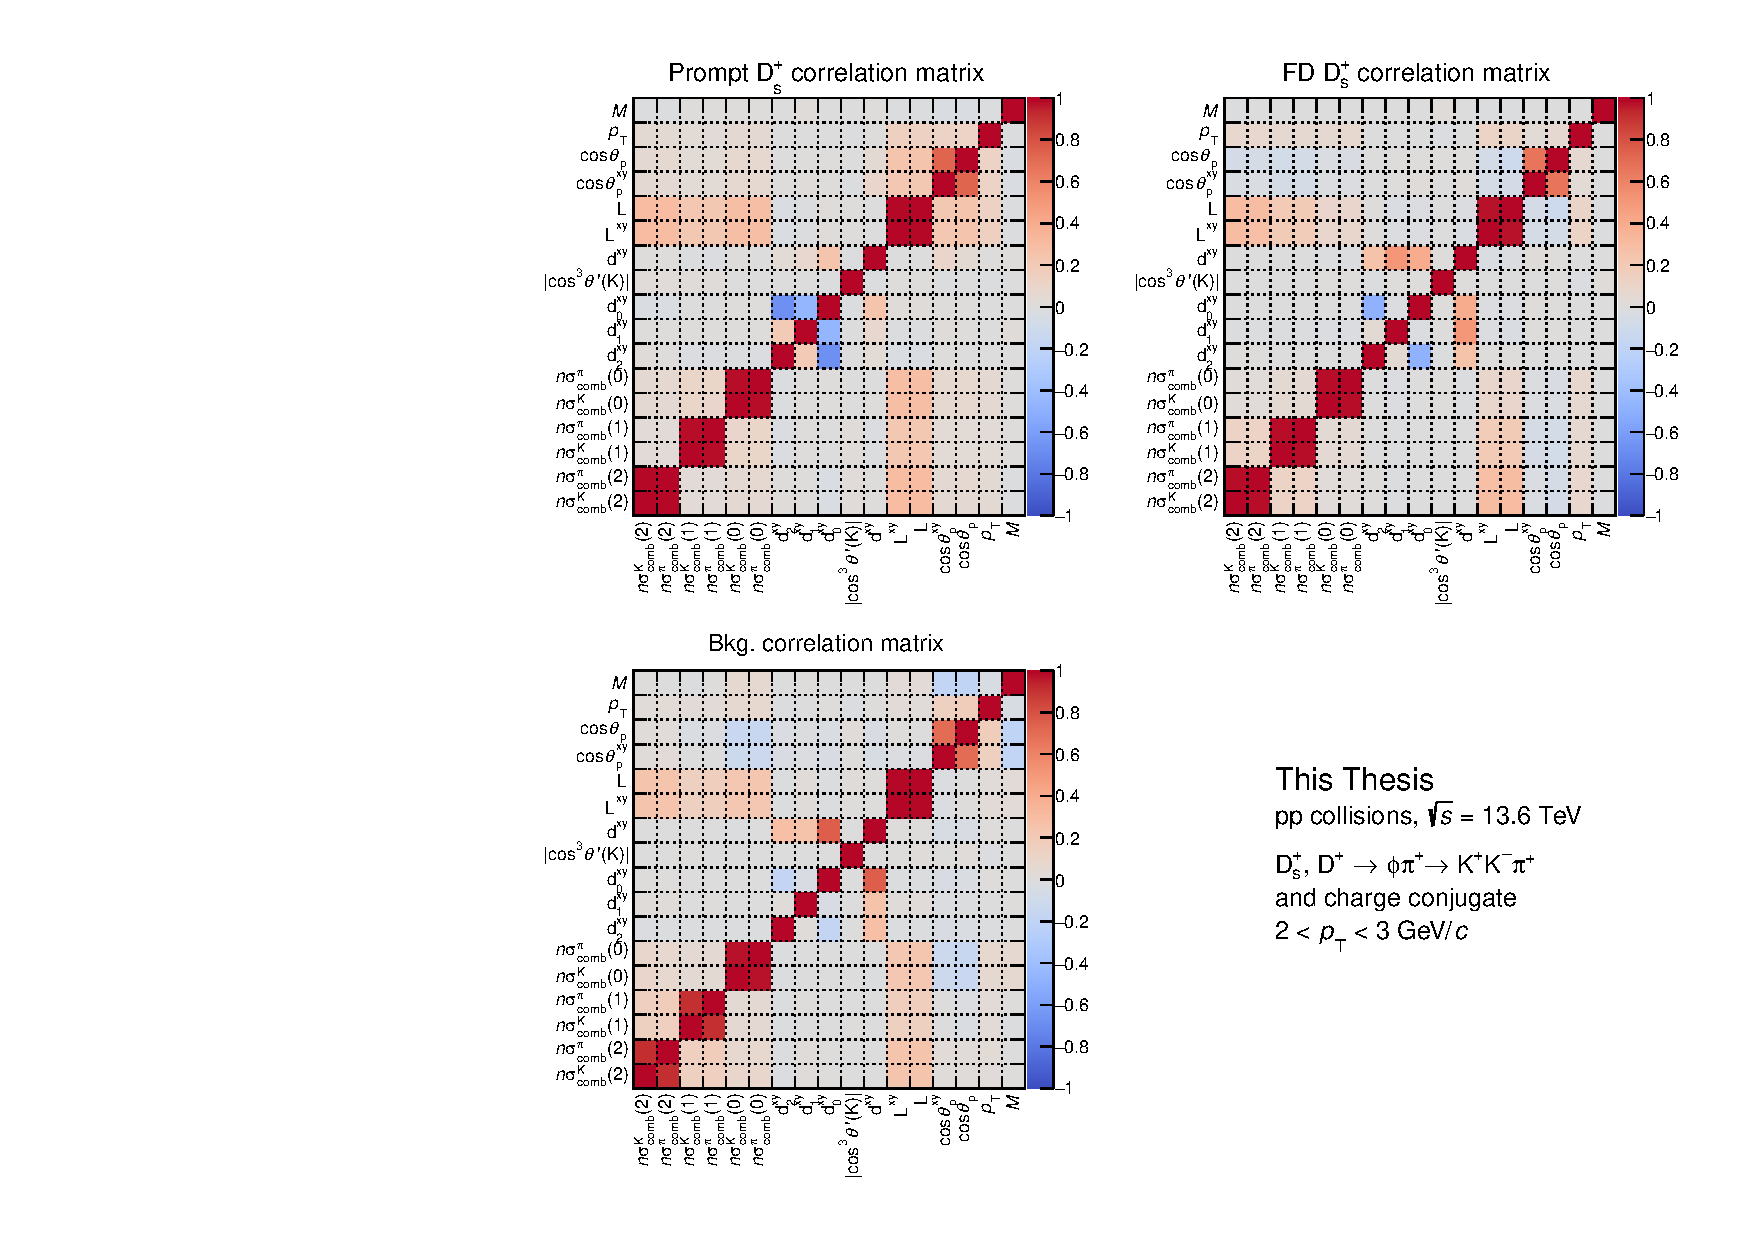
\includegraphics[width=\textwidth]{Figures/Chapter 5/CorrelationMatrix.pdf}
    \caption{Correlation matrix of the features used to train the ML model for prompt \ds (top-left), non-prompt \ds (top-right), and background (bottom-left) candidates in the $2<\pt<3$~\gevc interval. The correlation with the invariant mass and the transverse momentum is also reported. The Pearson coefficient is encoded in the colour of the cell, with red indicating a positive correlation, blue a negative correlation, and grey no linear correlation.}
    \label{fig:ml_training_vars}
\end{figure}

\subsection{Boosted Decision Trees}
Once the training dataset has been composed, and the features have been selected, the ML architecture has to be chosen. Several algorithms are available, each with its own strengths and weaknesses. The choice of the algorithm depends on the specific problem to solve, the size of the dataset, and the computational resources available. 

Boosted decision trees~\cite{friedman2001greedy,freund1997decision} (BDTs) are a family of machine learning algorithms employed in different fields, including high-energy physics. Their building blocks are decision trees, which are a versatile type of supervised learning algorithm that can be used for both classification and regression tasks. A decision tree is made of many \emph{nodes}, each containing conditions that split the data into two~\cite{breiman2017classification} or more~\cite{quinlan1986induction} children nodes. The first node of the tree, which receives all the data, is called the \emph{root}, while nodes that do not further split the data are called \emph{leaves}, and contain the output of the tree. The model is trained by considering the Gini index, which measures the impurity of the node:
\begin{equation*}
    G = 1 - \sum_{i=1}^{n} p_{i}^{2}\quad ,
\end{equation*}
where $p_{i}$ is the fraction of samples in the node that belong to class $i$. The Gini index therefore provides an indication of the quality of the split. A commonly used algorithm to build \emph{binary} decision trees (i.e., each node contains binary-output conditions, and is split into two children nodes) is the \emph{Classification And Regression Tree} (CART) algorithm~\cite{breiman2017classification}, which recursively splits the dataset into subsets based on a single feature $k$ and a threshold $t_k$ that minimises the impurity of the subsets (weighted by their size). The cost function that the algorithm tries to minimise is given by
\begin{equation*}
    J(k,t_k) = \frac{m_{\mathrm{left}}}{m}G_{\mathrm{left}} + \frac{m_{\mathrm{right}}}{m}G_{\mathrm{right}}\quad ,
\end{equation*}
where $m_{\mathrm{left}}$ and $m_{\mathrm{right}}$ are the number of samples in the left and right nodes, respectively, summing up to the total number of samples $m$, and $G_{\mathrm{left}}$ and $G_{\mathrm{right}}$ are the Gini indices of the left and right nodes. The tree is grown until a stopping criterion is met, such as a maximum depth, a minimum number of samples in a node, or a minimum impurity decrease. These are all hyperparameters that can be tuned to optimise the model's performance.

Given their simplicity, decision trees are fairly easy to interpret, and are often called \emph{white-box} models (in contrast to BDTs and neural networks, where the decision-making process is less transparent, therefore called \emph{black-box} models). An additional strength of decision trees is that they require
very little data preparation, e.g., they do not require feature scaling or centering, making them a very powerful yet simple tool for data analysis. However, they are prone to overfitting, as they can grow to a large depth, capturing the noise in the training data. To mitigate this issue, their depth is usually constrained, but this may lead to a model with limited discrimination power. To build a robust model with a good discrimination power, ensemble methods may be used. Several decision trees can be trained, and the final prediction is obtained by combining the outcome of all the trees. 

\subsubsection{XGBoost}
In this work, the Extrame Gradient Boosting~\cite{DBLP:xgboost} (XGBoost) Boosted Decision Trees (BDT) algorithm is used. It has achieved state-of-the-art results in a number of machine learning and data mining challenges (for example in Ref.~\cite{kaggle:higgs}). In addition, this algorithm, which is available as an open-source package, can be easily parallelised on CPUs and GPUs~\cite{mitchell2017accelerating} reducing the training and application time.

The term \emph{boosting} refers to any ensemble method combining several weak learners into a strong learner. The general idea of most boosting methods is to train many predictors sequentially, each trying to correct its predecessor~\cite{geron2022hands}. The function estimate $\widehat{f}(\mathbf{x})$ is parametrised with an additive functional form:
\begin{equation*}
    \widehat{f}(x) = \sum_{\mathrm{k}=1}^{\mathrm{M}} \widehat{f}_\mathrm{k}(x)\quad ,
\end{equation*}
where $M$ is the number of iterations, $\widehat{f}_\mathrm{0}(x)$ is the initial prediction, and $\widehat{f}_\mathrm{i}(x)$ is the function increment at the $i$-th iteration, also called \emph{boost}. To reduce the loss function, a new weak learner, whose functional form is parametrised as $h(\mathbf{x},\theta)$, can be added to the ensemble:
\begin{equation*}
    \widehat{f}_\mathrm{t}(\mathbf{x}) \leftarrow \widehat{f}_{\mathrm{t}-1}(\mathbf{x}) + \rho_\mathrm{t} h(\mathbf{x},\theta_\mathrm{t})\quad ,
\end{equation*}
$\rho_t$ is the step size, which is optimised for each iteration t, together with the parameters $\theta_\mathrm{t}$ of the weak learner:
\begin{equation*}
    (\rho_\mathrm{t}, \theta_\mathrm{t}) = \arg\min_{\rho,\theta} \sum_{{i}=1}^{\mathrm{N}} L\left(y_i, \widehat{f}_{\mathrm{t}-1}(x_i) + \rho h(x_i,\theta)\right)\quad ,
\end{equation*}
where $L$ is the loss function, and $y_i$ is the true label of the i-th example. Despite having a well-defined set of equations for minimising the loss function, the optimisation of the parameters is not trivial, as the loss function is non-convex and the search space is high-dimensional. Therefore, the optimisation is usually performed using a gradient-based algorithm~\cite{friedman2001greedy,natekin2013gradient}, where $h(\mathbf{x},\theta_\mathrm{t})$ is chosen as the most parallel function to the negative gradient of the loss function with respect to the previous prediction $g_\mathrm{t}(\mathbf{x})$:
\begin{equation*}
    g_\mathrm{t}(\mathbf{x}) = E_{\mathbf{y}}\left[ \frac{\partial L(\mathbf{y},\widehat{f}_{\mathrm{t}-1}(\mathbf{x}))}{\partial \widehat{f}_{\mathrm{t}-1}(\mathbf{x})} \Bigg{|} \mathbf{x} \right] \quad ,
\end{equation*}
where $E_{\mathbf{y}}$ is the expectation over the true labels. The parameters are then optimised by minimising the difference between the negative gradient and the weak learner prediction:
\begin{equation*}
    (\rho_\mathrm{t}, \theta_\mathrm{t}) = \arg\min_{\rho,\theta} \sum_{\mathrm{i}=1}^{\mathrm{N}} \left[-g_\mathrm{t} - \rho h(x_\mathrm{i},\theta)\right]^{2}\quad .
\end{equation*}

Through the iterative addition of weak learners, the model is able to learn complex patterns in the data, and to reduce the loss function. The final prediction is obtained by summing the predictions of all the weak learners. In the XGBoost algorithm, the weak learners are decision trees.

\subsection{Tuning the model's hyperparameters}
The XGBoost algorithm has several hyperparameters~\cite{XGBoost_parameters} that can be tuned to optimise the model's performance. The most important hyperparameters are:
\begin{itemize}
    \item \code{eta} or \code{learning\_rate}, which is the step size shrinkage of the gradient descent algorithm. To reduce the risk of overfitting, this factor multiplies the weak-learner prediction ($\rho_\mathrm{t} h(x_\mathrm{i},\theta) \rightarrow \code{eta} \cdot \rho_\mathrm{t} h(x_\mathrm{i},\theta)$), and is usually set to a small value, such as 0.3;
    \item \code{max\_depth}, which is the maximum depth of the tree. A large depth can lead to overfitting, while a small depth can lead to a model with limited discrimination power;
    \item \code{n\_estimators}, which defines the number of trees to train. A large number of weak learners can lead to overfitting, while a small number can lead to a model with limited discrimination power. Usually, the number of weak learners is set to around 1000;
    \item \code{subsample}, which is the fraction of the training data to be used to train each tree at each iteration;
    \item \code{min\_child\_weight}, which is the minimum sum of instance weight needed in a child. It is related to the purity in a node, and it is used to stop the tree growth;
    \item \code{colsample\_bytree}, which is the fraction of features to be used to train each tree at each iteration;
    \item \code{tree\_method}, which defines the algorithm used to build the trees. The \code{hist} option uses an optimised histogram-based algorithm and is usually the fastest.
\end{itemize}

The hyperparameters are optimised using the Optuna framework~\cite{akiba2019optuna}, which proved to be a powerful tool thanks to its state-of-the-art algorithms for sampling the hyperparameter space and for efficiently pruning unpromising trials. The Tree-Structured Parzen Estimator~\cite{bergstra2011algorithms}, is used in this Thesis. It is a Bayesian optimisation~\cite{frazier2018tutorial,snoek2012practical} algorithm able to explore the hyperparameter space efficiently. The aim of a Bayesian optimisation is to maximise (or minimise, depending on the task) an objective function $f(\mathbf{x})$ by iteratively sampling a bounded hyperparameter space, $\chi$. The algorithm builds a probabilistic model of the objective function, and uses it to decide which hyperparameters to sample next. The model is updated at each iteration, and the hyperparameters that are most likely to improve the model's performance are sampled. The Optuna algorithm is also able to prune unpromising trials, reducing the computational cost of the optimisation. The optimisation is performed using a 5-fold cross-validation, and the hyperparameters that maximise the macro-averaged one-vs-one ROC AUC metric (described in detail in Sec.~\ref{sec:ml_performance}) are chosen as the optimal configuration. The hyperparameters optimised for the XGBoost model are reported in Table~\ref{tab:ml_hyperparameters}. An additional hyperparameter, \code{lambda}, which is the L2 regularisation term, is also optimised. It helps to prevent overfitting by penalising overly complex models. The optimal hyperparameters are then used to train the model on the full training dataset.

\begin{table}[tb!]
    \centering
    \caption{Optimised hyperparameter configuration for the \pt bins considered in the model training.}
    \label{tab:ml_hyperparameters}
    \vspace*{0.3cm}
    \resizebox{\columnwidth}{!}{%
    \begin{tabular}{c|ccccccccc}
         \toprule
         Hyper-parameter & \multicolumn{9}{c}{$\pt$ interval (\gevc)} \\
         \midrule
          & 0--1.5 & 1.5--2 & 2--3 & 3--4 & 4--5 & 5--6 & 6--8 & 8--12 & 12--24 \\
        \midrule
         \code{max\textunderscore depth} & 3 & 3 & 3 & 3 & 3 & 3 & 3 & 3 & 3\\

         \code{learning\textunderscore rate} & 0.04 & 0.068 & 0.065 & 0.10 & 0.091 & 0.84 & 0.070 & 0.046 & 0.030\\
         
         \code{n\textunderscore estimators} & 473 & 339 & 1352 & 909 & 1256 & 1392 & 1142 & 1437 & 1188\\ 
         
         \code{min\textunderscore child\textunderscore weight} & 1 & 3 & 10 & 10 & 10 & 9 & 3 & 7 & 5\\
         
         \code{subsample} & 0.87 & 0.95 & 0.84 & 0.85 & 0.95 & 0.85 & 0.81 & 0.94 & 0.88\\
         
         \code{colsample\textunderscore bytree} & 0.91 & 0.98 & 0.90 & 0.98 & 0.96 & 0.95 & 0.88 & 0.96 & 0.89\\

         \code{lambda} & $8.0\times10^{-4}$ & $4.8\times10^{-4}$ & $9.1\times10^{-4}$ &  $1.4\times10^{-4}$  &  $3.0\times10^{-4}$ & $3.2\times10^{-4}$ & $1.9\times10^{-4}$ & $9.8\times10^{-4}$ & $6.7\times10^{-4}$\\
         $\code{tree\textunderscore method}$ & $\code{hist}$ & $\code{hist}$ & $\code{hist}$ & $\code{hist}$& $\code{hist}$& $\code{hist}$ & $\code{hist}$ & $\code{hist}$& $\code{hist}$\\
         \bottomrule
    \end{tabular}%
}
\end{table}

\subsection{Evaluation of the model's performance}\label{sec:ml_performance}
After training the model, its performance is evaluated on the test dataset. The model's performance can be assessed using a \emph{confusion matrix}, which summarises the number of examples for a given class (the true label) that are classified by the model as belonging to any of the available classes (the predicted label). A good model should provide a high number of correctly-classified examples (reported on the diagonal of the confusion matrix), and a low number of misclassified examples (off-diagonal elements of the confusion matrix). The confusion matrix also allows an understanding of which classes are more difficult to classify, and which classes are more likely to be confused with each other. An example of confusion matrix for the XGBoost model trained on the $2<\pt<3$~\gevc interval is shown in Fig.~\ref{fig:ml_confusion_matrix}.

\begin{figure}
    \centering
    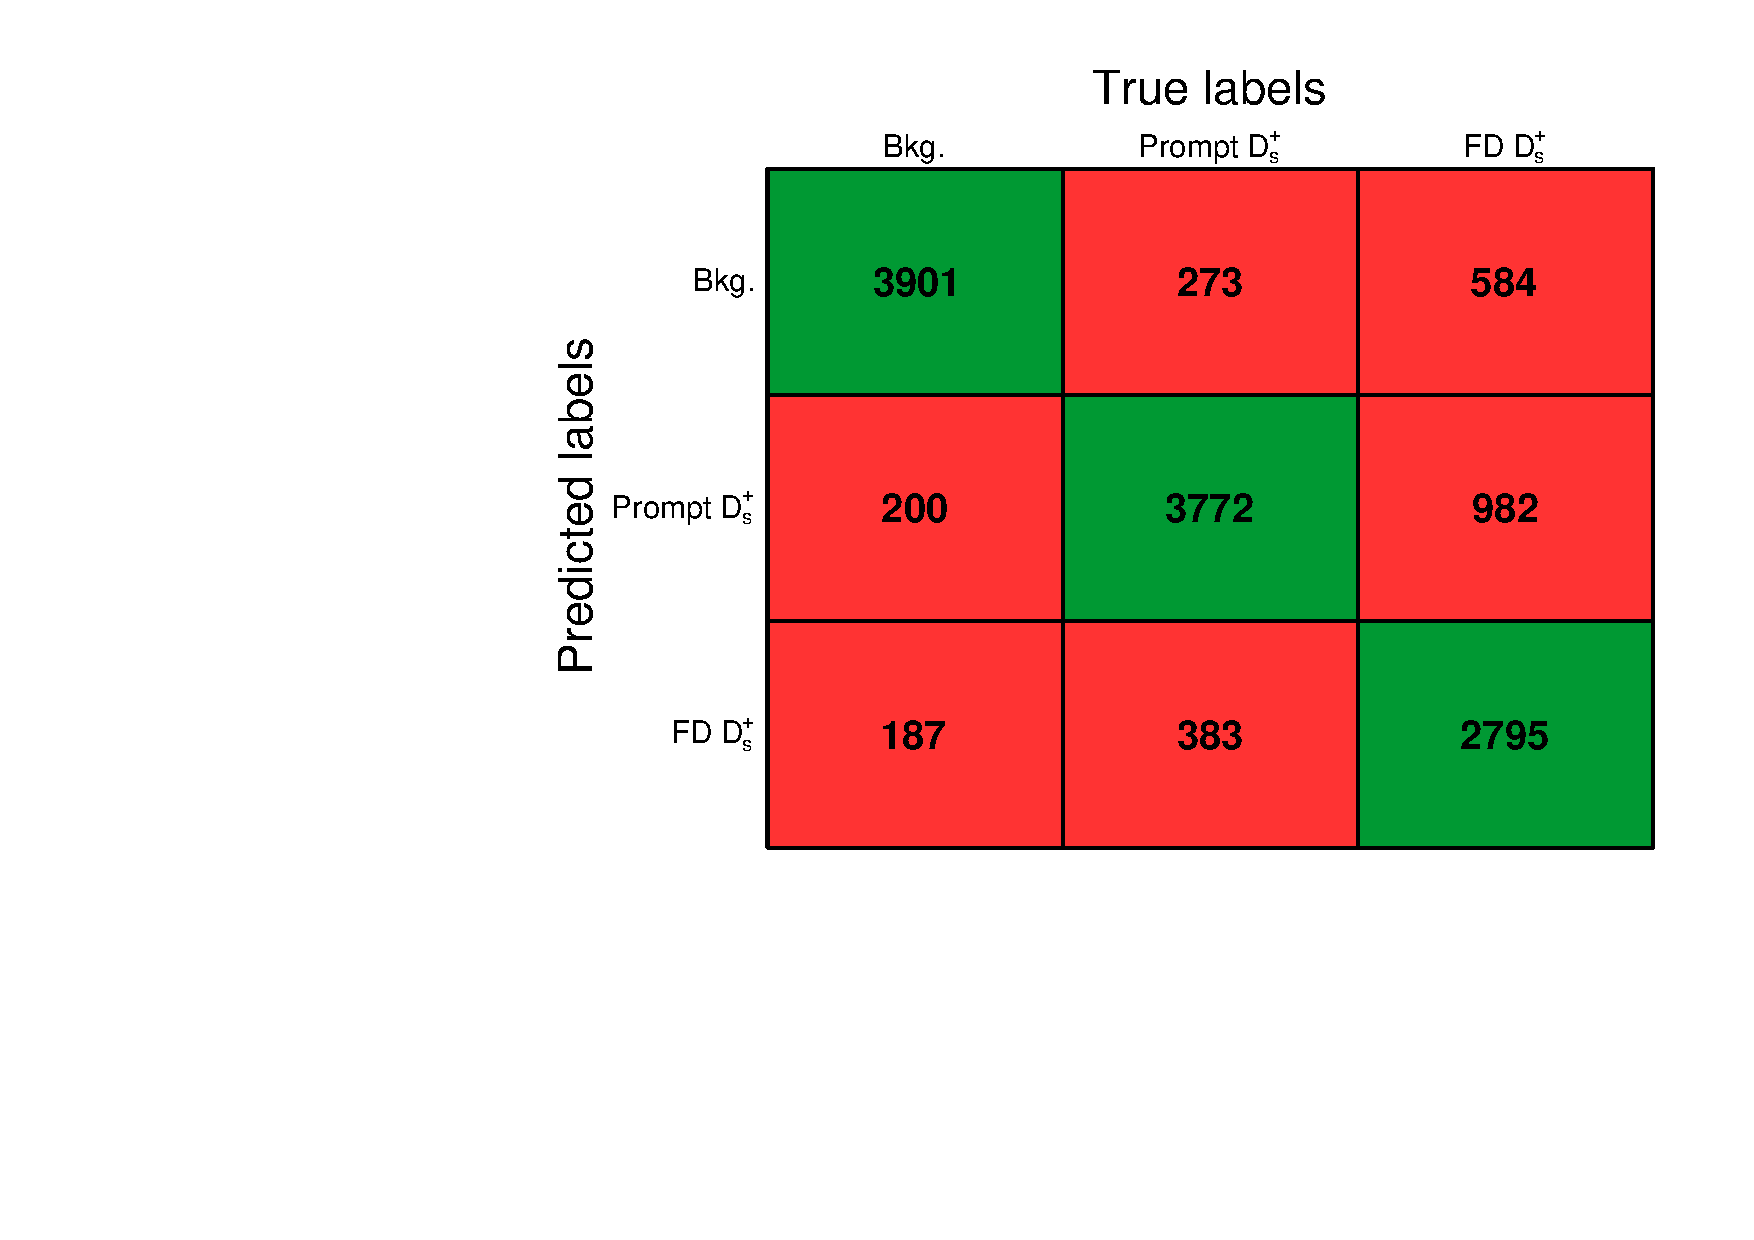
\includegraphics[width=0.7\textwidth]{Figures/Chapter 5/ConfusionMatrix.pdf}
    \caption{Confusion matrix for the XGBoost model trained on the $2<\pt<3$~\gevc interval. The classes are assigned as follows: if a candidate score is less than 0.5, it is classified as background; if it is greater than 1.5, it is classified as non-prompt \ds, and it is classified as prompt \ds otherwise.}
    \label{fig:ml_confusion_matrix}
\end{figure}

Despite providing a lot of information on the model's performance, more concise metrics of the model's performance are usually used, for a more direct comparison between different models. In addition, the confusion matrix provides a threshold-dependent measure of the model's performance, as the classification threshold can be varied to increase the number of correctly classified signal candidates at the expense of the number of correctly classified background candidates, and vice versa. 

In binary classification tasks, where only two classes are available (a positive and a negative class), several metrics can be defined from the elements of the confusion matrix. The $2\mkern-2mu\times\mkern-2mu2$ confusion matrix contains four entries: the true positives (TP), which are the number of correctly classified positive candidates, the false positives (FP), which are the number of negative candidates being mistakenly classified as positives, and the analogously defined true negatives (TN) and false negatives (FN). One of the most used tools for binary classifiers is the \emph{Receiver Operating Characteristic} (ROC) curve, which represents the true positive rate (TPR) against the false positive rate (FPR) for different threshold values. The TPR is the fraction of correctly classified positive candidates ($\mathrm{TPR = TP/(TP+FN)}$), while the FPR is the fraction of incorrectly classified negative candidates ($\mathrm{FPR = FP/(FP+TN)}$). If positive candidates are selected as those with a score greater than a certain threshold $t$, then when $t=0$ all candidates are classified as positive, and both the TPR and FPR will be equal to 1. On the other hand, if $t=1$, no candidate is classified as positive, and the TPR and FPR will both equal 0. The ROC \emph{Area Under the Curve} (AUC), is used to measure the model's ability to discriminate between positive and negative candidates, for any given threshold. The ROC AUC ranges from 0 to 1. A random classifier has a ROC AUC of 0.5, while a perfect classifier has a ROC AUC of 1. The ROC AUC is a threshold-independent measure of the model's performance, and is used to compare different models. 

In a multiclass classification task, where more than two classes are available, the ROC curve and the ROC AUC cannot be used. In this case, the ROC curve can be generalised to the \emph{One-vs-One} ROC curve, which is a plot of the TPR against the FPR for each class. The ROC AUC can be averaged to the \emph{macro-averaged} One-vs-One ROC AUC, which is the average of the ROC AUC for each pair of classes and can provide a measurement of the model's ability to discriminate between all the classes.


The ROC curves for the model trained on the $2<\pt<3$~\gevc interval are shown in Fig.~\ref{fig:ml_roc_curve}. The One-vs-One ROC AUC is calculated for each class pair, and is reported in the legend. The metric is evaluated on both the training and test sets to test the model's generalisation power. The model's performance is excellent, with a macro-averaged One-vs-One ROC AUC value close to 1. In addition, little overfitting is observed, as the ROC AUC values for the training and test sets are similar. The model is then used to select \ds and \dpl candidates from the full dataset. 

\begin{figure}[htb]
    \centering
    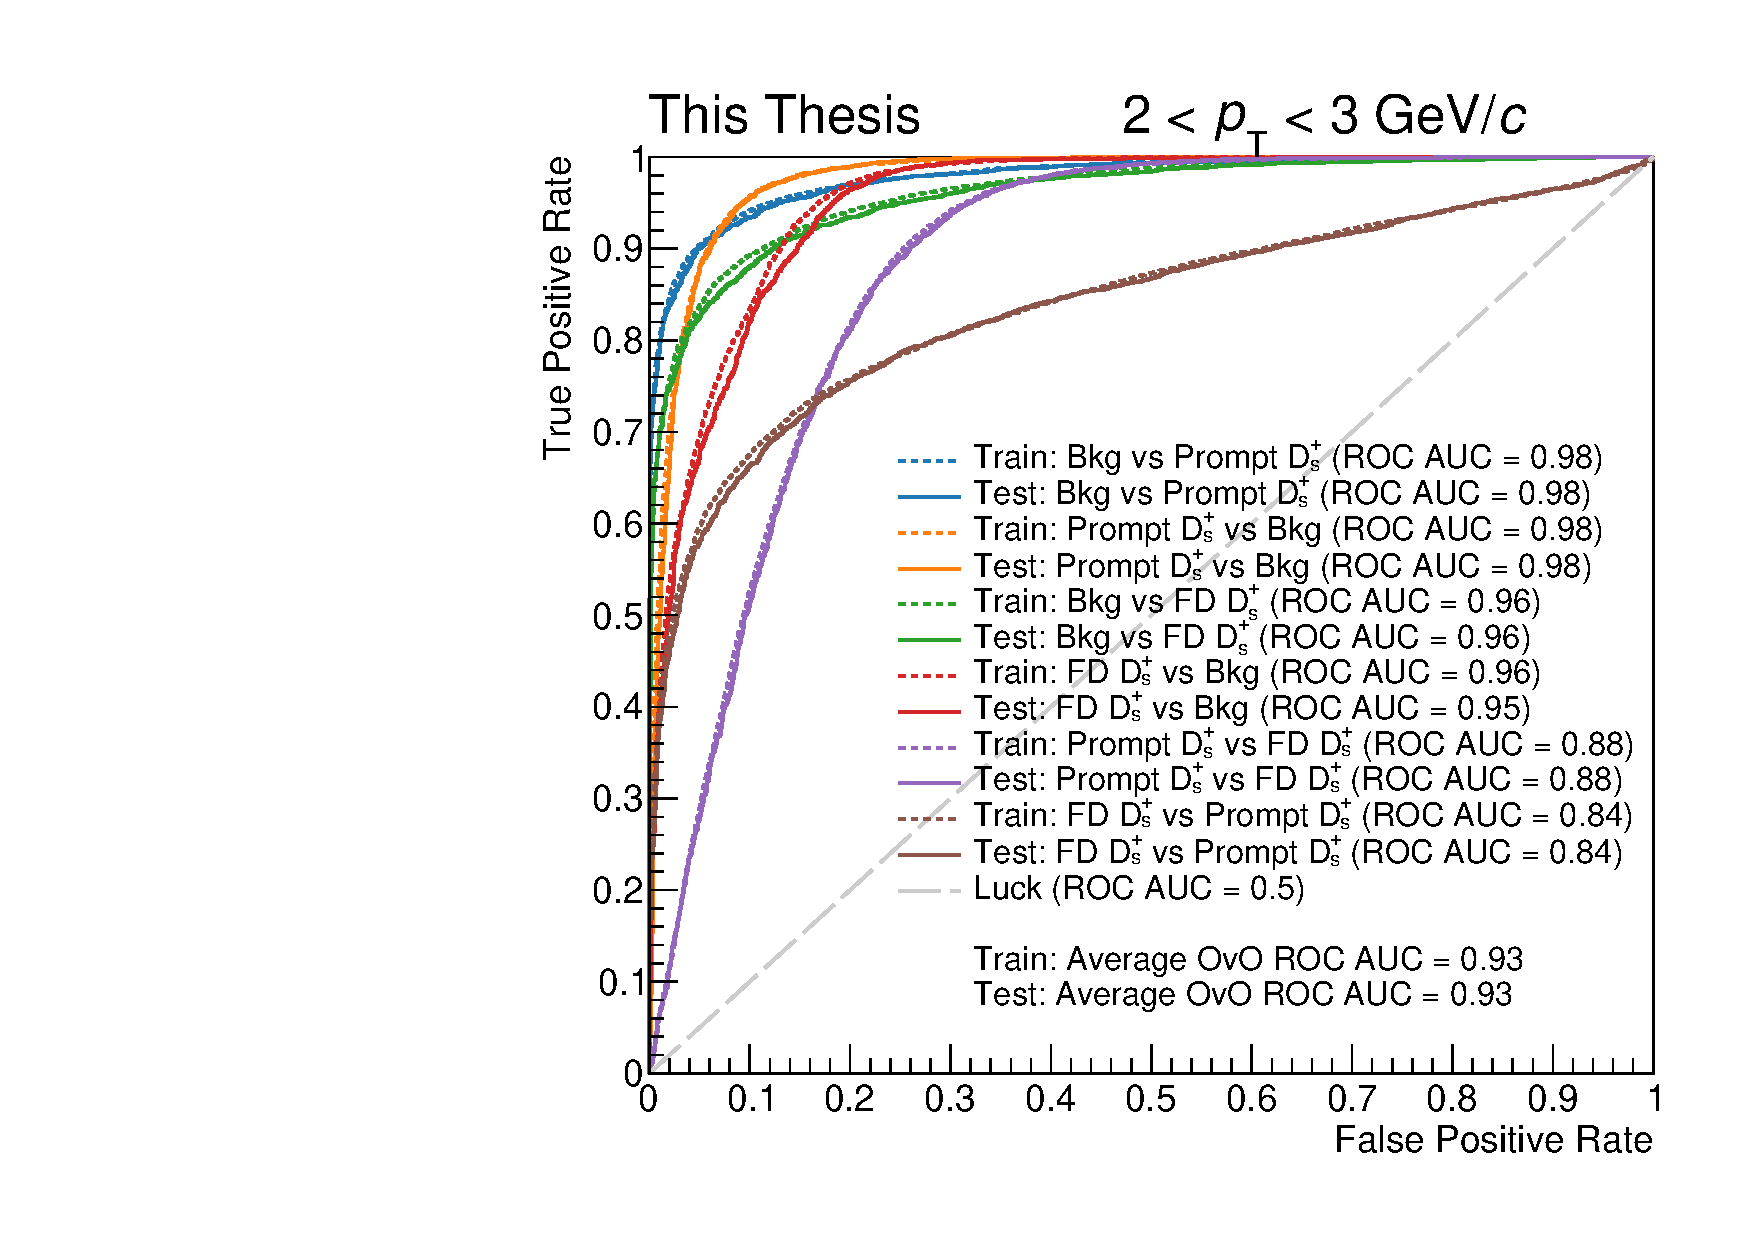
\includegraphics[width=0.7\textwidth]{Figures/Chapter 5/ROC.pdf}
    \caption{ROC curves for the model trained on the $2<\pt<3$~\gevc interval. The One-vs-One ROC AUC metric is calculated for each class pair and reported in the legend.}
    \label{fig:ml_roc_curve}
\end{figure}

\begin{sloppypar}
In addition to the ROC AUC, the model's performance can be evaluated by studying the distribution of the probability of belonging to a given class assigned to labelleled candidates. The score distribution for the model trained on the \mbox{$2<\pt<3$~\gevc} interval is shown in Fig.~\ref{fig:ml_score} for the background, prompt \ds, and non-prompt \ds classes. For each class, the score distribution is shown for candidates belonging to the different classes and to both the training and test sets. The distribution of the background score provides interesting information on the model's performance. The score distribution for the background candidates peaks at high values, while the score distribution for the signal candidates (both prompt and non prompt \ds) peaks at low values. This highlights that the model has effectively learned to discriminate between signal and background candidates, with good separation power. Furthermore, the score distributions for the training and test sets are fairly similar, indicating that the model generalises well to unseen data. Since non-prompt \ds present a very displaced topology due to the large lifetime of beauty-hadrons, the separation between non-prompt \ds and background is noticeable in the non-prompt \ds score distribution. Finally, as the displacement of prompt candidates lies in between the non-prompt \ds and background, the separation between the three classes is less pronounced in the prompt \ds score distribution, where the prompt \ds distribution does not peak at values around one.
\end{sloppypar}

\begin{figure}[p]
    \centering
    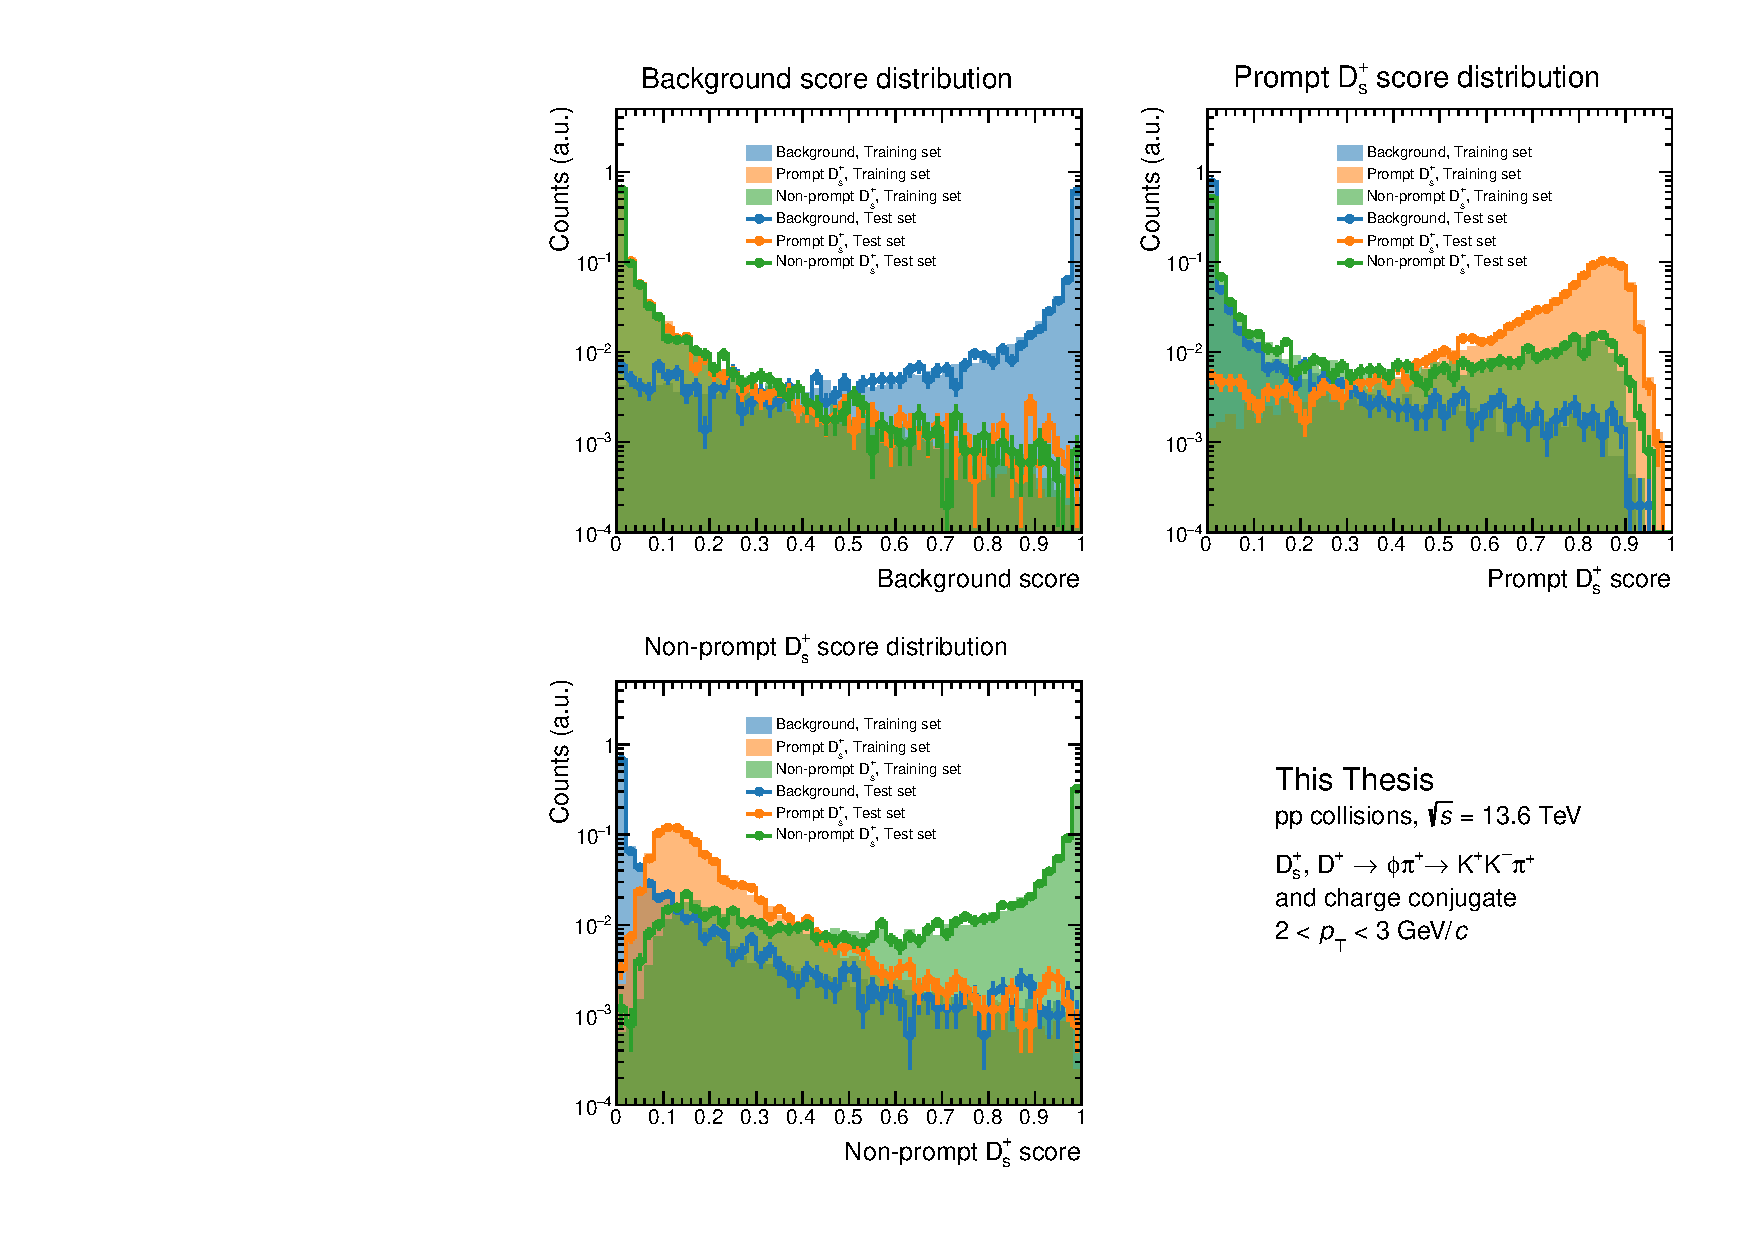
\includegraphics[width=\textwidth]{Figures/Chapter 5/Distributions.pdf}
    \caption{Score distribution for the model trained on the $2<\pt<3$~\gevc interval. The score distribution related to the probability of belonging to the background, prompt \ds, and non-prompt \ds classes is shown. For each class, the score distribution is shown for candidates belonging to the different classes and to both the training (filled area) and test sets (markers).}
    \label{fig:ml_score}
\end{figure}

\subsection{Interpretation of the model's output: Feature importance}
The usage of ML algorithms usually provides a better performance in terms of signal-to-background separation, but it also introduces a level of complexity in the selection process. One of the most difficult aspects of using ML models is the interpretation of their output. To understand how the model makes its decisions, the feature importance can be studied. This allows the understanding of which features are more important for the model's decision-making process, and the optimisation of the feature selection. In addition, the feature importance can be used to check whether the model is learning on the correct features in terms of the physics of the problem.

One of the most used algorithms for feature importance studies is the SHapley Additive exPlanations~\cite{lundberg2017unified} (SHAP) algorithm. SHAP is a game-theoretic approach to explain the output of any machine learning model. It is based on the Shapley value~\cite{lipovetsky2001analysis} from cooperative game theory, which requires retraining the model on all feature subsets $\mathcal{S}\subseteq \mathcal{F}$, where $\mathcal{F}$ is the set of all features. An importance value is assigned to each feature, representing the effect on the model prediction of including that feature. To compute this effect, a model $\widehat{f}_{\mathcal{S}\cup\{i\}}$ is trained with that feature present, and another model $\widehat{f}_\mathcal{S}$ is trained with the feature withheld. Then, predictions from the two
models are compared on the current input $\widehat{f}_{\mathcal{S}\cup\{i\}} (x) - \widehat{f}_\mathcal{S}$. The Shapley values are then computed as the weighted average of all possible differences:
\begin{equation*}
    \phi_\mathrm{i} = \sum_{\mathcal{S}\subseteq \mathcal{F}\setminus\{i\}} \frac{|\mathcal{S}|!(|\mathcal{F}|-|\mathcal{S}|-1)!}{|\mathcal{F}|!} \left[\widehat{f}_{\mathcal{S}\cup\{i\}}(x) - \widehat{f}_\mathcal{S}(x)\right]\quad .
\end{equation*}
Since most models cannot handle arbitrary patterns of missing input values, $\widehat{f} (z_\mathcal{S})$ is approximated with $E[\widehat{f}(z) | z_\mathcal{S}]$, where $z_\mathcal{S}$ is the input missing the features in $\mathcal{S}$. SHAP values therefore explain how to get from the base value E[f(z)] that would be predicted if no features were known to the output f(x).

A beeswarm-style SHAP feature importance plot for the prompt \ds probability predicted by the model trained in the $2<\pt<3$~\gevc interval is shown in Fig.~\ref{fig:ml_feature_importance}. The most important features are the cosine of pointing angle, the decay length, the decay length in the XY plane, the cosine cubed of the K-$\pi$ angle in the KK rest frame, and the PID information on the prong 1. As discussed in Chapter~\ref{chap:reconstruction}, the first three features are related to the displaced topology of D mesons, and are therefore expected to be the most important variables in the model decisions. Iit is also expected that the prong 1 PID information resulted as the important PID variable, as this is the opposite sign track, which is always a kaon in the considered decay channel. On the contrary, prongs 0 and 2 could either be kaons or pions, resulting in a lower importance of the PID information for these prongs. 

\begin{figure}[htb]
    \centering
    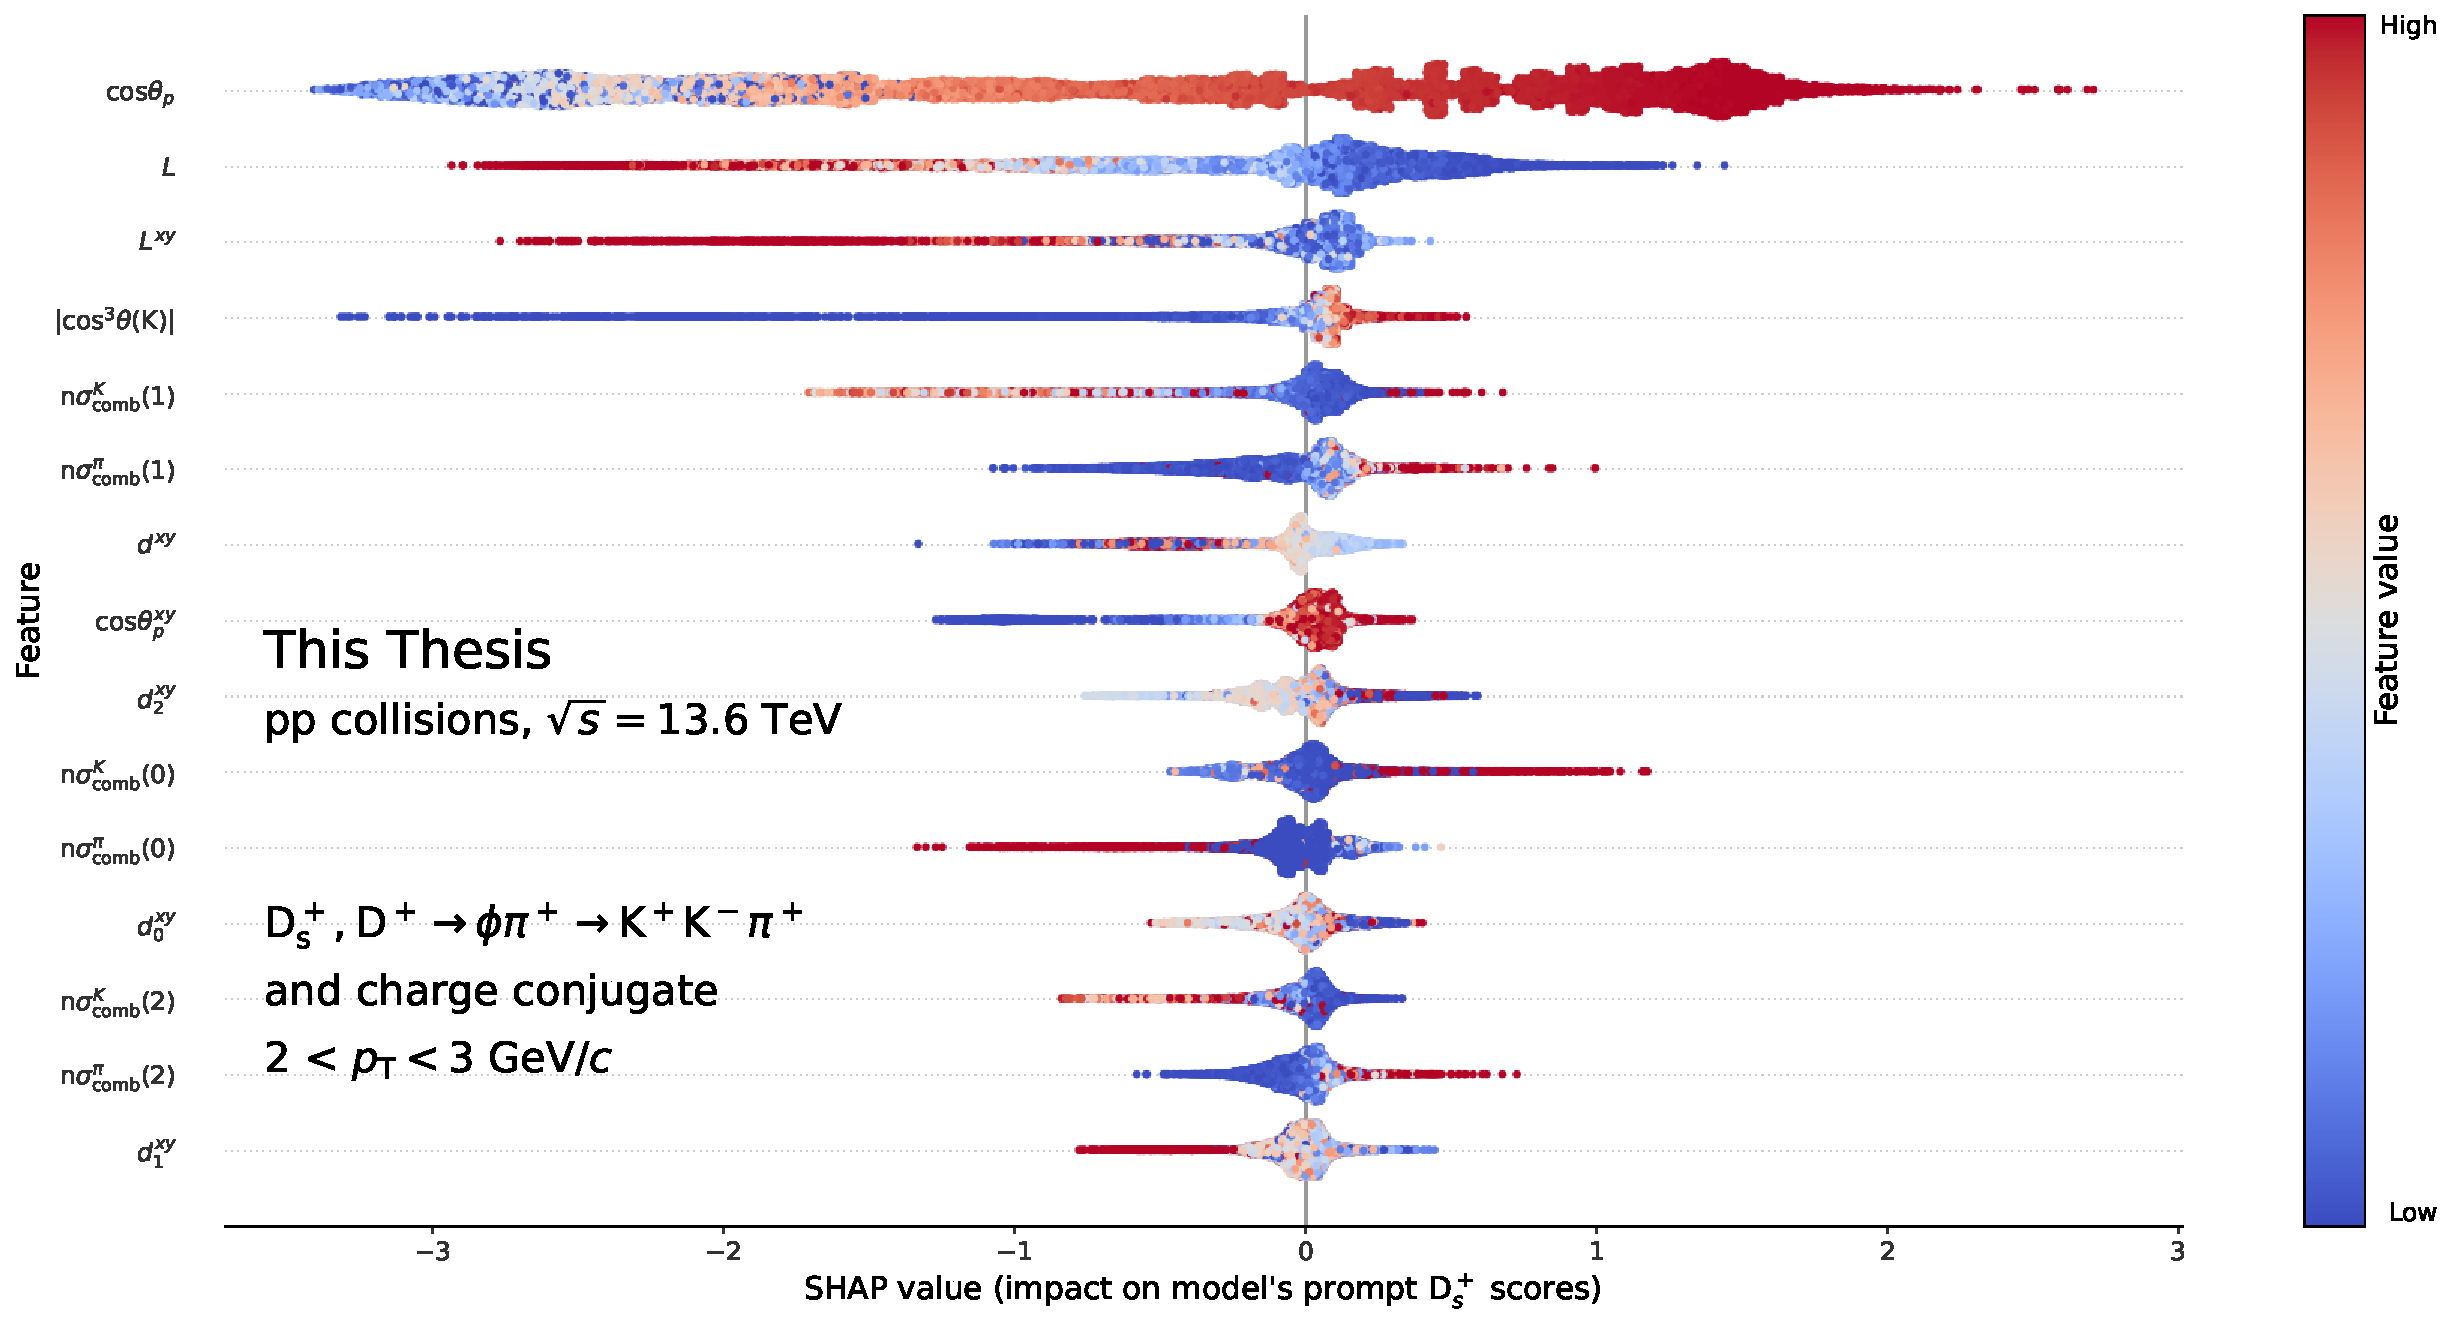
\includegraphics[width=\textwidth]{Figures/Chapter 5/shap.pdf}
    \caption{SHAP feature importance for the XGBoost model trained on the $2<\pt<3$~\gevc interval.}
    \label{fig:ml_feature_importance}
\end{figure}

\subsection{Optimisation of the model selection}
Once the model performance has been validated, a set of selection criteria has to be chosen to select the candidates. 